\documentclass[graduacao,brazil]{ThesisPUC}
\usepackage{float}
\usepackage{enumerate}

%%%%%%%%%%%%%%%%%%%%%%%%%%%%%%%%%%%%%%%%%%%%%%%%%%%%%%%%%%%%%%%%%%%%%%%%%%%%%%%%

\newcommand{\Rset}{\mathbb{R}}
\newcommand{\Zset}{\mathbb{Z}}

%%%%%%%%%%%%%%%%%%%%%%%%%%%%%%%%%%%%%%%%%%%%%%%%%%%%%%%%%%%%%%%%%%%%%%%%%%%%%%%%

\autor{Julio Ribeiro da Silva}
\autorR{Silva, Julio Ribeiro da}
\orientador{S\'{e}rgio Lifschitz}
\orientadorR{Lifschitz, S\'{e}rgio}

\titulo{PrISMA}
\titulouk{PrISMA}
\subtitulo{Programa de Instru\c{c}\~{a}o \`{a} Solicita\c{c}\~{a}o de Matr\'{i}cula Acad\^{e}mica}
\dia{09} \mes{Abril} \ano{2014}

\cidade{Rio de Janeiro}
\CDD{510}
\departamento{Inform\'atica}
\programa{Engenharia da Computa\c{c}\~{a}o}
\centro{Centro T\'{e}cnico Cient\'{i}fico}
\universidade{Pontif\'{i}cia Universidade Cat\'{o}lica do Rio de Janeiro}
\uni{PUC--Rio}
\course{Engenharia da Computa\c{c}\~{a}o}
\diploma{Bacharel em Engenharia da Computa\c{c}\~{a}o}

%%%%%%%%%%%%%%%%%%%%%%%%%%%%%%%%%%%%%%%%%%%%%%%%%%%%%%%%%%%%%%%%%%%%%%%%%%%%%%%%

  \agradecimentos{%
Primeiramente, à minha família, que esteve comigo durante todos os momentos da minha vida e tornaram possível eu chegar até aqui.

Em segundo lugar, à Luiza Noronha, que foi quem esteve ao meu lado durante todo o desenvolvimento deste projeto. Assim como ao meu orientador, Sérgio Lifschitz, a quem eu atribuo a autoria da ideia, e que também tornou a sua implantação possível. Também àqueles que fizeram parte de alguma etapa do seu desenvolvimento. 

Ao professor Luiz Fernando Bessa Seibel, que me acolheu em seu laboratório durante pouco mais de três anos e sempre acreditou em mim.

À todos aqueles que estiveram ao meu lado durante toda a minha graduação que, além de compartilhar experiências acadêmicas, também compartilharam experiências pessoais.

E, não menos importante, aos alunos da PUC-Rio que utilizaram o PrISMA. Sem vocês este projeto não teria o sucesso que foi alcançado.

Cada um de vocês foi importante neste processo. Muito obrigado.
}


%%%%%%%%%%%%%%%%%%%%%%%%%%%%%%%%%%%%%%%%%%%%%%%%%%%%%%%%%%%%%%%%%%%%%%%%%%%%%%%%

 \chaves{%
   \chave{Banco de dados}%
   \chave{Experi\^{e}ncia do usu\'{a}rio}%
   \chave{Aplica\c{c}\~{a}o web}%
   \chave{API REST}%
 }
 
 \resumo{
Na PUC-Rio, no início de cada período os alunos informam quais turmas gostariam de cursar, de acordo com os seus planejamentos. No entanto, dado que o número de vagas por turmas é limitado, na maior parte das vezes não é possível atender a todos os pedidos de todos os alunos. Este problema que o PrISMA se propõe a minimizar. Através de uma aplicação web bastante poderosa, e ao mesmo tempo de fácil uso, auxiliar os alunos passo a passo nas suas decisões na hora de montar o seu planejamento de turmas para o período seguinte.
 }
 
 
% %%%%%%%%%%%%%%%%%%%%%%%%%%%%%%%%%%%%%%%%%%%%%%%%%%%%%%%%%%%%%%%%%%%%%%%%%%%%%%%%
 
 \chavesuk{
   \chave{Database}%
   \chave{User Experience}%
   \chave{Web application}%
   \chave{REST API}%
 }
 
 \resumouk{%
At PUC-Rio, in the beginning of each period students tells which classes they would like to attend, according to their schedules. However, given that the number of vacancies for classes is limited, in most cases it is not possible to attend all requests for all students. This is the problem PrISMA aims to minimize. Through a very powerful and easy to use web application assist students step by step in their decisions when scheduling classes for the following period.
 }


%%%%%%%%%%%%%%%%%%%%%%%%%%%%%%%%%%%%%%%%%%%%%%%%%%%%%%%%%%%%%%%%%%%%%%%%%%%%%%%%

\modotabelas{nada} % nada, fig, tab ou figtab

%%%%%%%%%%%%%%%%%%%%%%%%%%%%%%%%%%%%%%%%%%%%%%%%%%%%%%%%%%%%%%%%%%%%%%%%%%%%%%%%

\begin{document}

%%%%%%%%%%%%%%%%%%%%%%%%%%%%%%%%%%%%%%%%%%%%%%%%%%%%%%%%%%%%%%%%%%%%%%%%%%%%%%%%

\chapter{Introdu\c{c}\~ao}

A Pontifícia Universidade Católica do Rio de Janeiro (PUC-Rio) oferece a seus alunos diversos cursos de graduação, cujas disciplinas são contabilizadas e disponibilizadas em um sistema de contagem de créditos. Os alunos precisam conter em seus históricos escolares um número mínimo de créditos pertencentes a um determinado currículo de um curso para que obtenham seus diplomas. 

Assim, e ao longo de sua vida universitária, os alunos da PUC-Rio buscam organizar os semestres escolares e escolhas de disciplinas de forma que consigam se formar no menor tempo possível. Apenas alunos calouros não fazem escolhas de disciplinas (e respectivos créditos). A partir do segundo período de seu curso, cada aluno da PUC-Rio deve escolher quais disciplinas para o novo período escolar pretende cursar.

As decisões sobre a escolha de disciplinas são baseadas na oferta de disciplinas daquele período, nos pré-requisitos e compatibilidade de horários. Há também de se considerar turmas distintas de mesmas disciplinas, horários conflitantes, limite no total de vagas oferecidas por turma e total de créditos permitido por semestre. Há também preferências (ou impedimentos) de caráter pessoal, como é o caso de alunos que têm outras atividades (e.g. estágio em empresas ou laboratórios acadêmicos) em paralelo com suas vidas acadêmicas. Cabe observar que a PUC-Rio determina prioridades em relação à ocupação de vagas de acordo com uma ordenação interna que pondera basicamente o desempenho acadêmico do aluno (C.R. – coeficiente de rendimento), a quantidade de créditos já obtidos, consequentemente, o tempo estimado para completar os créditos necessários para concluir o curso.

A PUC-Rio requisita, a cada semestre, que os alunos preparem uma solicitação de matrícula com três opções contendo o conjunto de disciplinas e turmas que pretende cursar no semestre seguinte. Esta escolha é chamada de grade: disciplinas, dias e horários escolhidos em função da lista de turmas oferecidas pela Universidade para o período seguinte. Há restrições de montagem da grade, como por exemplo, um valor máximo de horas (ou créditos) semanais, turma de matérias distintas par a par; e turmas cujos horários não conflitem entre si, ou seja, que tenham os horários disjuntos, também par a par.

Caso a primeira opção de um aluno não seja totalmente atendida, por exemplo, por falta de vaga, o sistema de matrícula tenta incluir as disciplinas escolhidas em segunda ou terceira opção, buscando atender os pedidos de um aluno. É fato que muitos alunos não se dão por satisfeitos pois muitas disciplinas solicitadas ficam de fora da seleção final de disciplinas efetivamente matriculadas inicialmente. Sem o apoio de uma ferramenta adequada, os ajustes de matrícula em disciplinas, realizados a cada início de semestre escolar, se tornaram cada vez mais frequentes. Entre outros motivos, uma das razões que fazem com que os alunos não fiquem satisfeitos com sua grade de disciplinas escolar diz respeito às decisões equivocadas no momento de solicitação e da montagem da grade de opções.

Consequentemente, a PUC-Rio deve alocar mais recursos para tentar resolver a situação individual de cada aluno pós-solicitação, os alunos precisam comparecer, muitas das vezes, pessoalmente para tentar corrigir suas grades e todo o processo fica mais complicado, e com resultados, muitas das vezes, indesejáveis. Implicando assim em perdas para ambas as partes.

%%%%%%%%%%%%%%%%%%%%%%%%%%%%%%%%%%%%%%%%%%%%%%%%%%%%%%%%%%%%%%%%%%%%%%%%%%%%%%%%

\chapter{Estado da Arte}

Para auxiliar os alunos na montagem da grade há um grande esforço por parte da PUC-Rio na orientação de como deve ser feito o procedimento de solicitação de matrícula. Este, por sua vez, deve ser realizado através do site da universidade, por meio de uma interface que dá margem a diversas interpretações quanto ao seu funcionamento.

Muitos alunos, por sua vez, buscam se informar e combinar com seus colegas para montar a melhor grade possível, montando planilhas e fazendo simulações do que poderia acontecer caso suas solicitações não fossem atendidas. Infelizmente esta abordagem implica em uma quantidade de trabalho muito grande, e em cima de interpretações muitas das vezes incorretas de como o processo deveria ser feito.

Diversas críticas e discussões acerca do modelo como um todo são feitas. No entanto, nenhuma solução concreta havia sido proposta ainda. De acordo com o apresentado até o momento, o problema persiste.

%%%%%%%%%%%%%%%%%%%%%%%%%%%%%%%%%%%%%%%%%%%%%%%%%%%%%%%%%%%%%%%%%%%%%%%%%%%%%%%%

\chapter{Solução proposta}

Propõe-se então o sistema PrISMA (Programa de Instrução à Solicitação de Matrícula acadêmica). Trata-se de uma aplicação web que reúne todas as funcionalidades necessárias para auxiliar os alunos no processo de matrícula.

O objetivo do sistema é apresentar uma interface muito poderosa, reunindo todos os dados necessários à solicitação, e ao mesmo tempo intuitiva, de forma que os alunos não fiquem perdidos durante o processo. Isso se faz necessário pois o processo como um todo exige o acesso à muita informação ao mesmo tempo, tornando o desenvolvimento do projeto um grande desafio.

O básico, para os alunos, seria reunir num mesmo ambiente seu Falta Cursar, disciplinas oferecidas pelo Micro Horário e as disciplinas já selecionadas para a grade do próximo período. Assim como uma visualização daquilo de já foi selecionado no formato de tabela de horários semanal. Dessa maneira, não seria mais necessário se perder no meio de diversas aplicações em busca de todas essas informações. Tudo estaria reunido em um único lugar.

Além da preocupação com a navegação, existe também a preocupação com a corretude da grade gerada. Por especificação, todas (ou pelo menos a maioria) das regras que impedem a solicitação de disciplinas devem ser implementadas. Sendo a principal delas a regra de pré-requisitos. Para tal, se faz necessário do histórico de disciplinas cursadas dos alunos, e do seu C.R. acumulado. Dessa maneira, conforme o aluno for utilizando e selecionando as disciplinas a serem cursadas, o sistema realiza a verificação e informa o aluno em caso de algum problema.

Buscando diminuir a quantidade de dados apresentados, ao invés de exibir as disciplinas do Falta Cursar do aluno, é précomputado o conjunto de disciplinas chamado de Pode Cursar. Este subconjunto contém apenas as disciplinas que não estão presas por nenhum pré-requisito. 

Olhando do ponto de vista das múltiplas opções no campo de solicitação, identifica-se uma grande incompreensão por parte dos alunos dessa funcionalidade no sistema da PUC. Essa falta de clareza se trata de uma das principais fontes de erros dos alunos na hora de preencher a solicitação. Por se tratar de um ponto crítico, propõe-se uma funcionalidade que, passo a passo, mostre ao usuário o que aconteceria caso alguma disciplina, de alguma opção fosse rejeitada, e que impacto isso teria no restante da solicitação.

Após terem suas grades montadas, deve-se preencher manualmente no site da PUC-Rio os dados gerados, já que se trata de um sistema independente. Uma solução para isto seria a definição de um padrão de arquivo exportado pelo PrISMA que fosse aceito pelo PUC Online (setor responsável pelo sistema da PUC-Rio). Entretanto, por se tratar de procedimentos burocráticos, não será de fato implementado pela PUC.

Para aqueles que oferecem as disciplinas é interessante ter dados estatísticos de uso do sistema por parte dos alunos. Apresentações de gráficos de lotação das turmas e como se comportam os alunos ao realizar o procedimento de escolha. Dessa maneira pode-se aprender com a necessidade dos alunos.

%%%%%%%%%%%%%%%%%%%%%%%%%%%%%%%%%%%%%%%%%%%%%%%%%%%%%%%%%%%%%%%%%%%%%%%%%%%%%%%%

\chapter{Projeto}

Nesta etapa será apresentada a estratégia utilizada no desenvolvimento do sistema. Aproveitando-se do fato de que o domínio do problema já foi apresentado e de que o objetivo a ser alcançado está bem definido.

Por enquanto, é de conhecimento geral que o resultado do projeto será uma aplicação web, onde os alunos terão acesso e poderão realizar todas as operações online. No entanto, na verdade são necessários muitos passos para se alcançar este objetivo. Por isso este tópico será abordado em três etapas:

\section{Design}

A parte mais importante de um sistema que interage diretamente com o público se chama experiência do usuário, e é muito simples enxergar isso. Quando um sistema extremamente poderoso se torna ao mesmo tempo extremamente complexo de ser utilizado, apenas os usuários mais dedicados farão uso dele. Caso apresentasse uma interface agradável aos olhos e de fácil compreensão, seria muito mais provável de que usuários menos dedicados também pudessem tirar proveito dos seus benefícios, contribuindo assim para a aceitação do sistema.

Com essa preocupação em mente que foi pensado o PrISMA. Tornar todas as funcionalidades e posicionamentos nas telas o mais óbvio possível, o que é um grande desafio, dado que são muitas as informações e possibilidades de interação que devem ser apresentadas aos usuários ao mesmo tempo.

Foi então feita uma parceria com um grupo do curso de Design (nota de rodapé: São eles: Gabriel Martinelli, Denis Neves, Glauber Borges e Maurício Fragale) da PUC-Rio que, por coincidência, já havia trabalhado na interface de um sistema com a mesma proposta. Já haviam feito estudo do caso e apresentado como projeto final de uma disciplina do curso deles e, dessa forma, criticada exaustivamente por seus professores. Dessa forma, foi apresentado o primeiro conceito do PrISMA.

\begin{figure}[H]
    \centering
    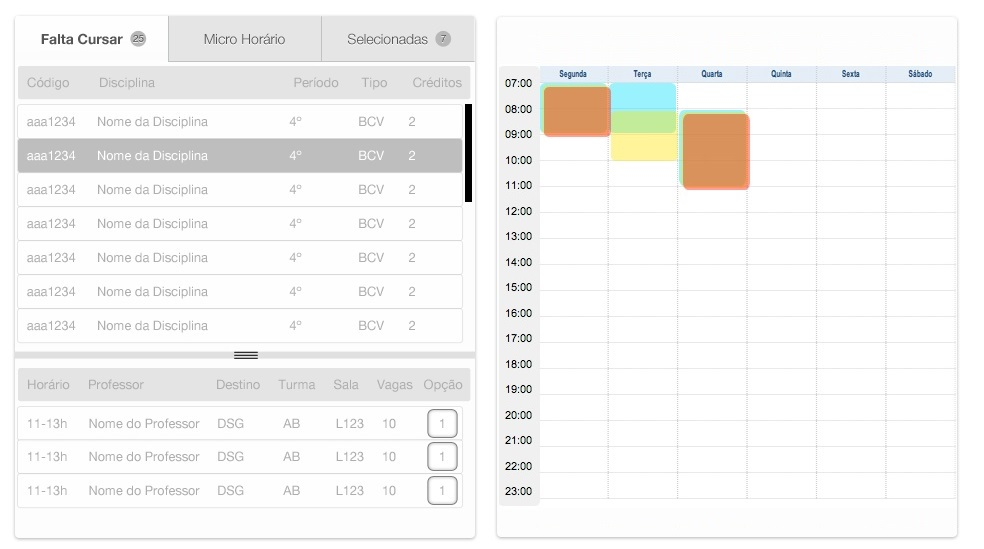
\includegraphics[width=\linewidth]{img/prisma.jpg}
    \caption{Primeira versão do layout.}
\end{figure}

Conforme a proposta original, é apresentado ao usuário durante toda a navegação uma tabela de horários por dias da semana. Com ela é possível visualizar claramente quais turmas estão sendo escolhidas, em quais horários e quais os conflitos entre elas.

No lado esquerdo ficariam localizados todos os dados necessários aos alunos, como seu Falta-Cursar, já filtrado pelas disciplinas que ele pode cursar (rodapé: Disciplinas ainda não cursadas que não estão presas por nenhum pré-requisito.), os dados das turmas disponibilizadas para o próximo período (Micro-Horário) e as turmas que foram selecionadas até o momento. Reunindo assim todos os dados em apenas um lugar. E se aproveitando do fato de que alguns dados não precisam, necessariamente, ser visualizados ao mesmo tempo que outros.

\section{Front-end}

Para que o projeto seja classificado como aplicação web deve-se tomar o cuidado para que a página carregada não seja recarregada por completo a cada interação do usuário, e que apenas os pontos de interesse assim o sejam. Dessa maneira, além de apresentar uma navegação mais fluida, há também a diminuição do trafego de dados no servidor, visto que ele não estará enviando a mesma informação várias vezes para um mesmo cliente.

Para tornar isso possível foram utilizadas as seguintes ferramentas:
\begin{itemize}
	\item \cite{Backbone} Framework MVC escrito em Javascript que tem por objetivo organizar a estrutura da aplicação, como persistência de dados, eventos, etc.
	\item \cite{Underscore} Biblioteca com diversas aplicações, mas a utilizada foi como controle dos templates utilizados. Isto é, controla a renderização de apenas parte da página.
	\item \cite{Bootstrap} Biblioteca de estilos CSS e controles em Javascript com o objetivo de auxiliar na implementação do design e comportamento das páginas.
	\item \cite{Jade} Linguagem que tem por objetivo facilitar a escrita do código HTML. Isto é, é uma linguagem que, quando compilada, gera HTML. Da mesma forma, na etapa de compilação pode-se solicitar que o HTML gerado tenha o menor tamanho possível, economizando assim no trafego de dados.
	\item \cite{Less} Atua da mesma maneira que o Jade, só que para o CSS. No entanto, com essa ferramenta é possível utilizar funções, variáveis, separar em arquivos, etc.
\end{itemize}

\section{Back-end}

Por se tratar de uma aplicação executada no navegador dos alunos, sem a necessidade de instalação, se faz necessário de um servidor para responder às requisições feitas. Assim como ele deve permitir que os usuários tenham acesso apenas aos seus dados, e não de outros, de modo a garantir segurança.

Para que as requisições sejam respondidas é necessário utilizar um servidor HTTP que, por ser de fácil configuração e conseguir lidar facilmente com uma grande quantidade de solicitações, foi escolhido o Apache HTTP Server.

Para tornar o conteúdo retornado sensível ao contexto se faz necessário utilizar uma linguagem para controlar as respostas. Nesta camada foi usada a linguagem PHP. No entanto, esta linguagem é muito permissiva quando se trata de desenvolvimento WEB, tornando extremamente necessário o uso de um framework. Dessa maneira, foi desenvolvido o Very Simple Rest Framework (nota de rodapé), exclusivamente para este projeto.

Para a persistência dos dados foi utilizado o banco de dados PostgreSQL. Ele foi escolhido por ser grátis, extremamente poderoso e garantir que não haveria perda de desempenho para diversas requisições simultâneas.

Com este conjunto de ferramentas é possível controlar todas as etapas de uma solicitação web por parte dos alunos, garantindo que seus dados estarão íntegros e seguros.

%%%%%%%%%%%%%%%%%%%%%%%%%%%%%%%%%%%%%%%%%%%%%%%%%%%%%%%%%%%%%%%%%%%%%%%%%%%%%%%%

\chapter{Planejamento}

Por se tratar de um sistema já implementado, a proposta para este projeto final de curso é de que seja feita a documentação do que já está pronto e a adição de algumas novas funcionalidades. São elas:

\begin{itemize}

  \item Como não existe integração do PrISMA com o PUC Online, os alunos precisam realizar a entrada de dados manualmente de um sistema para o outro. Para resolver este problema será então implementada uma exportação de dados, em um formato padronizado, de forma que a PUC aceite. Esta última etapa infelizmente não poderá ser cumprida, por motivos burocráticos.

  \item Até o momento foi apenas discutida a visão do aluno sobre o sistema. No entanto, serão agregados dados relevantes também àqueles que estão disponibilizando as turmas. Neste caso, estatísticas quanto à ocupação das turmas virão a ser oferecida.

  \item Da mesma forma, essas estatísticas podem ser apresentadas aos alunos para que possam ter uma ideia do quão concorrida será aquela vaga. Com isso, estes dados estarão disponíveis na visualização de cada turma.

  \item A cada novo período o PrISMA precisava ser configurado com os dados dos novos alunos, históricos de alunos antigos e novas turmas e disciplinas que serão oferecidas nos próximos períodos. Para isso se faz necessário que esses dados sejam carregados no sistema de alguma maneira. Como atualmente não existe uma interface de controle para este nível de administração, ela será implementada.
\end{itemize}

Por ser um sistema não tão pequeno, serão priorizadas as etapas de documentação do projeto. Dessa maneira, por mais que as funcionalidades sugeridas venham a ficar prontas, pelo menos algum outro desenvolvedor poderá continuar de onde foi parado. Dessa forma também será gerado um manual que poderá servir como referência no que se refere a desenvolvimento web, baseado na experiência adquirida.

Concluída a documentação, cada funcionalidade será avaliada e priorizada quanto à sua importância e tempo de implementação. Maximizando assim a proximidade do resultado obtido com a do esperado.

%%%%%%%%%%%%%%%%%%%%%%%%%%%%%%%%%%%%%%%%%%%%%%%%%%%%%%%%%%%%%%%%%%%%%%%%%%%%%%%%
\arial
\nocite{*}
\bibliography{relatorio1}

\normalfont

\end{document}
